Spatial decompositions of a set of $d$ dimensional coordinates into a single
dimension is widely applied across computational science. The spatial
decompositions of $d$ dimensional cubes especially finds a wide variety of applications,
from forming the basis of implementations of finite-element methods, to algorithms
for mesh refinement, and importantly in our case, $N$-body simulations
\cite{Sundar:2008:SIAM}. Spatial decompositions utilise space-filling curves,
these infinite-curves are fractal, and by increasing their `order' can be made
to `fill', or describe, a $d$ dimensional space uniquely, simply by their position
along the length of the curve \cite{Campbell:2003:Williams}. This concept is
illustrated in figure (\ref{fig:2_2_multi_order}) for the Morton encoding, or a
`Z-order' encoding, a variant of space-filling curves used in \gls{PyExaFMM}
that better preserves the proximality of data in the encoded coordinates than
 most other encodings, in addition to being easier to implement as it doesn't
 have the requirement that the encoded line has to be continuous.
 Figure (\ref{fig:2_2_multi_order}) illustrates the fractal nature of a Morton
 encoded line at two adjacent levels of a quadtree in two dimensions. The
 position along the line in each quadrant of a given box can be efficiently represented as a pair of `binary coordinates'
 corresponding to the index of the quadrant the line passes through for a given box.
 For example, the bottom-left quadrant at the coarser level in figure (\ref{fig:2_2_multi_order})
 will have a binary coordinate of $00$. This encoding can be made unique for each
 quadrant in each level by adding a displacement corresponding to the number of boxes so far
 encoded at all coarser levels. For example, the first encoded box, which in figure (\ref{fig:2_2_multi_order})
 corresponds to the binary coordinate $00$ will have a displacement due to the
 number of boxes thus far encoded at this level, and all coarser levels, of which
 there are none in this case, of 0. This leaves this first box with a Morton encoded position,
 or \textbf{\gls{key}} of 0 in base ten. Similarly, the encoding for the bottom-left box at the finer
 level in figure (\ref{fig:2_2_multi_order}) will have binary coordinates of $00$,
 and a displacement due to the number of boxes encoded at previous levels of 4
 \footnote{As is common in computer science, we begin indexing at 0, rather than 1.},
therefore it's Morton \gls{key} in base ten will be $4$.

This concept is easily extended to three dimensions, and is illustrated in
figure (\ref{fig:2_2_morton_encoding}) at level 1 of an octree. Here the binary
coordinates simply contain three bits, for the $xyz$ octant of a given cube
in the octree, and the displacement mechanism is entirely analogous with the
two dimensional case.

The binary coordinates of Morton encoded octant box make it easy to perform simple
bit shifts to find the parent box of a given box. To find a box's parent, all
one needs to do is subtract the displacement due to the number of boxes thus
far encoded, and perform a three bit shift to the 'right', removing the bits
corresponding to the encoded

- How PyExaFMM finds non-empty nodes (hilbert get keys from points)

- how to find children and parents

- how expansions are stored against keys

- Numba jitting

- Extensions work
    - parallel tree construction
    - adaptive trees


\begin{figure}[!h]
    \centering
    {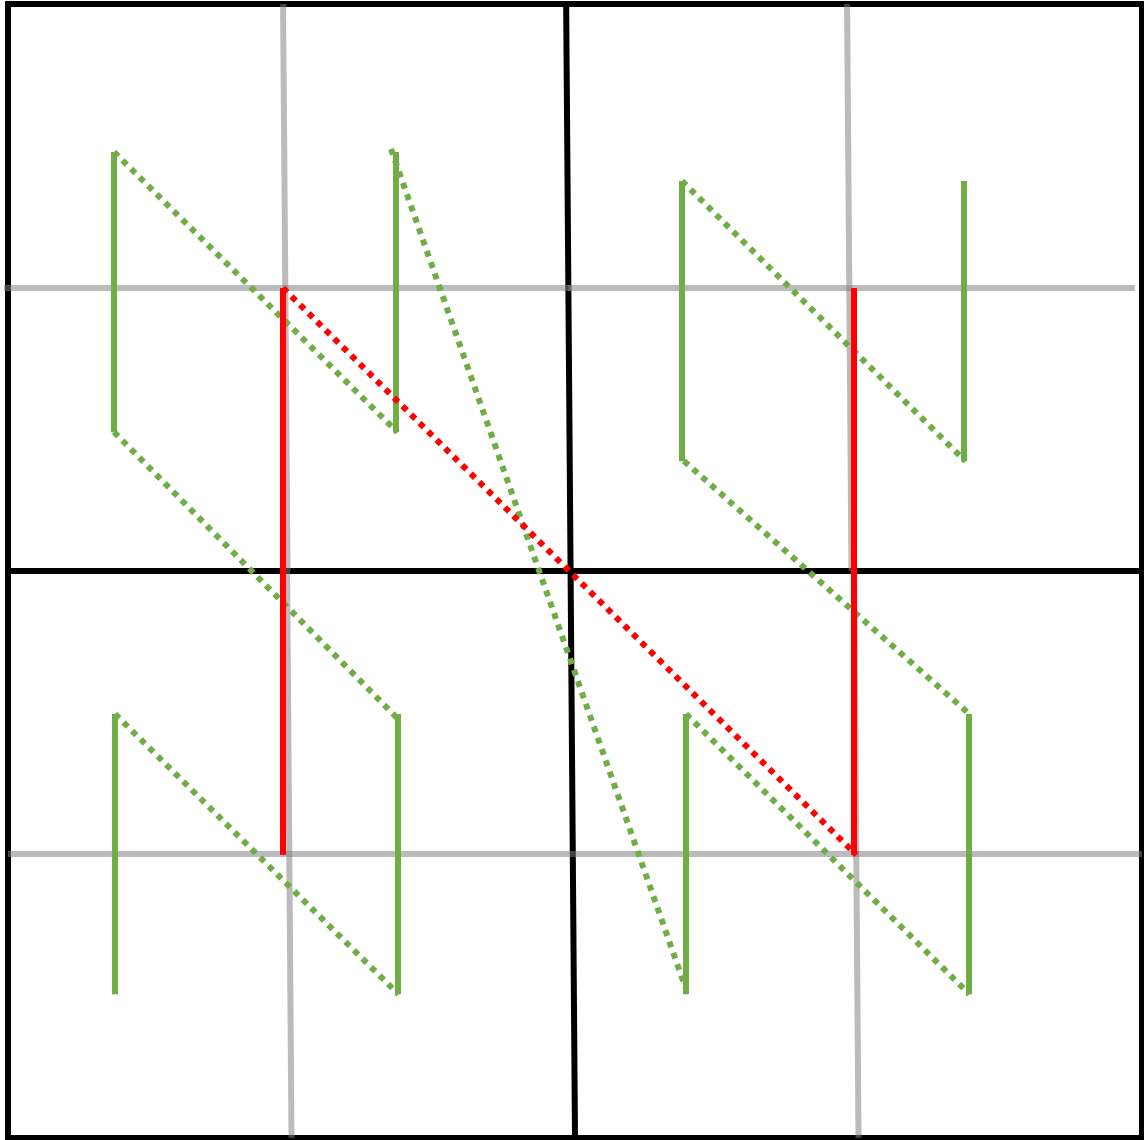
\includegraphics[width=0.45\textwidth]{chapter2/2_order.png}}
    \vspace{0pt}
    \caption{
        Two orders of Morton encoded lines in two dimensions for a quadtree across
        two adjacent levels. The red line encodes the center of the quadrants at the higher level,
        and and the green line encodes the corresponding points a level deeper.
        The dashed line indicates the order in which displacements are calculated
        in the encoding where the line is discontinuous.
    }
    \label{fig:2_2_multi_order}
\end{figure}


\begin{figure}[!h]
    \centering
    {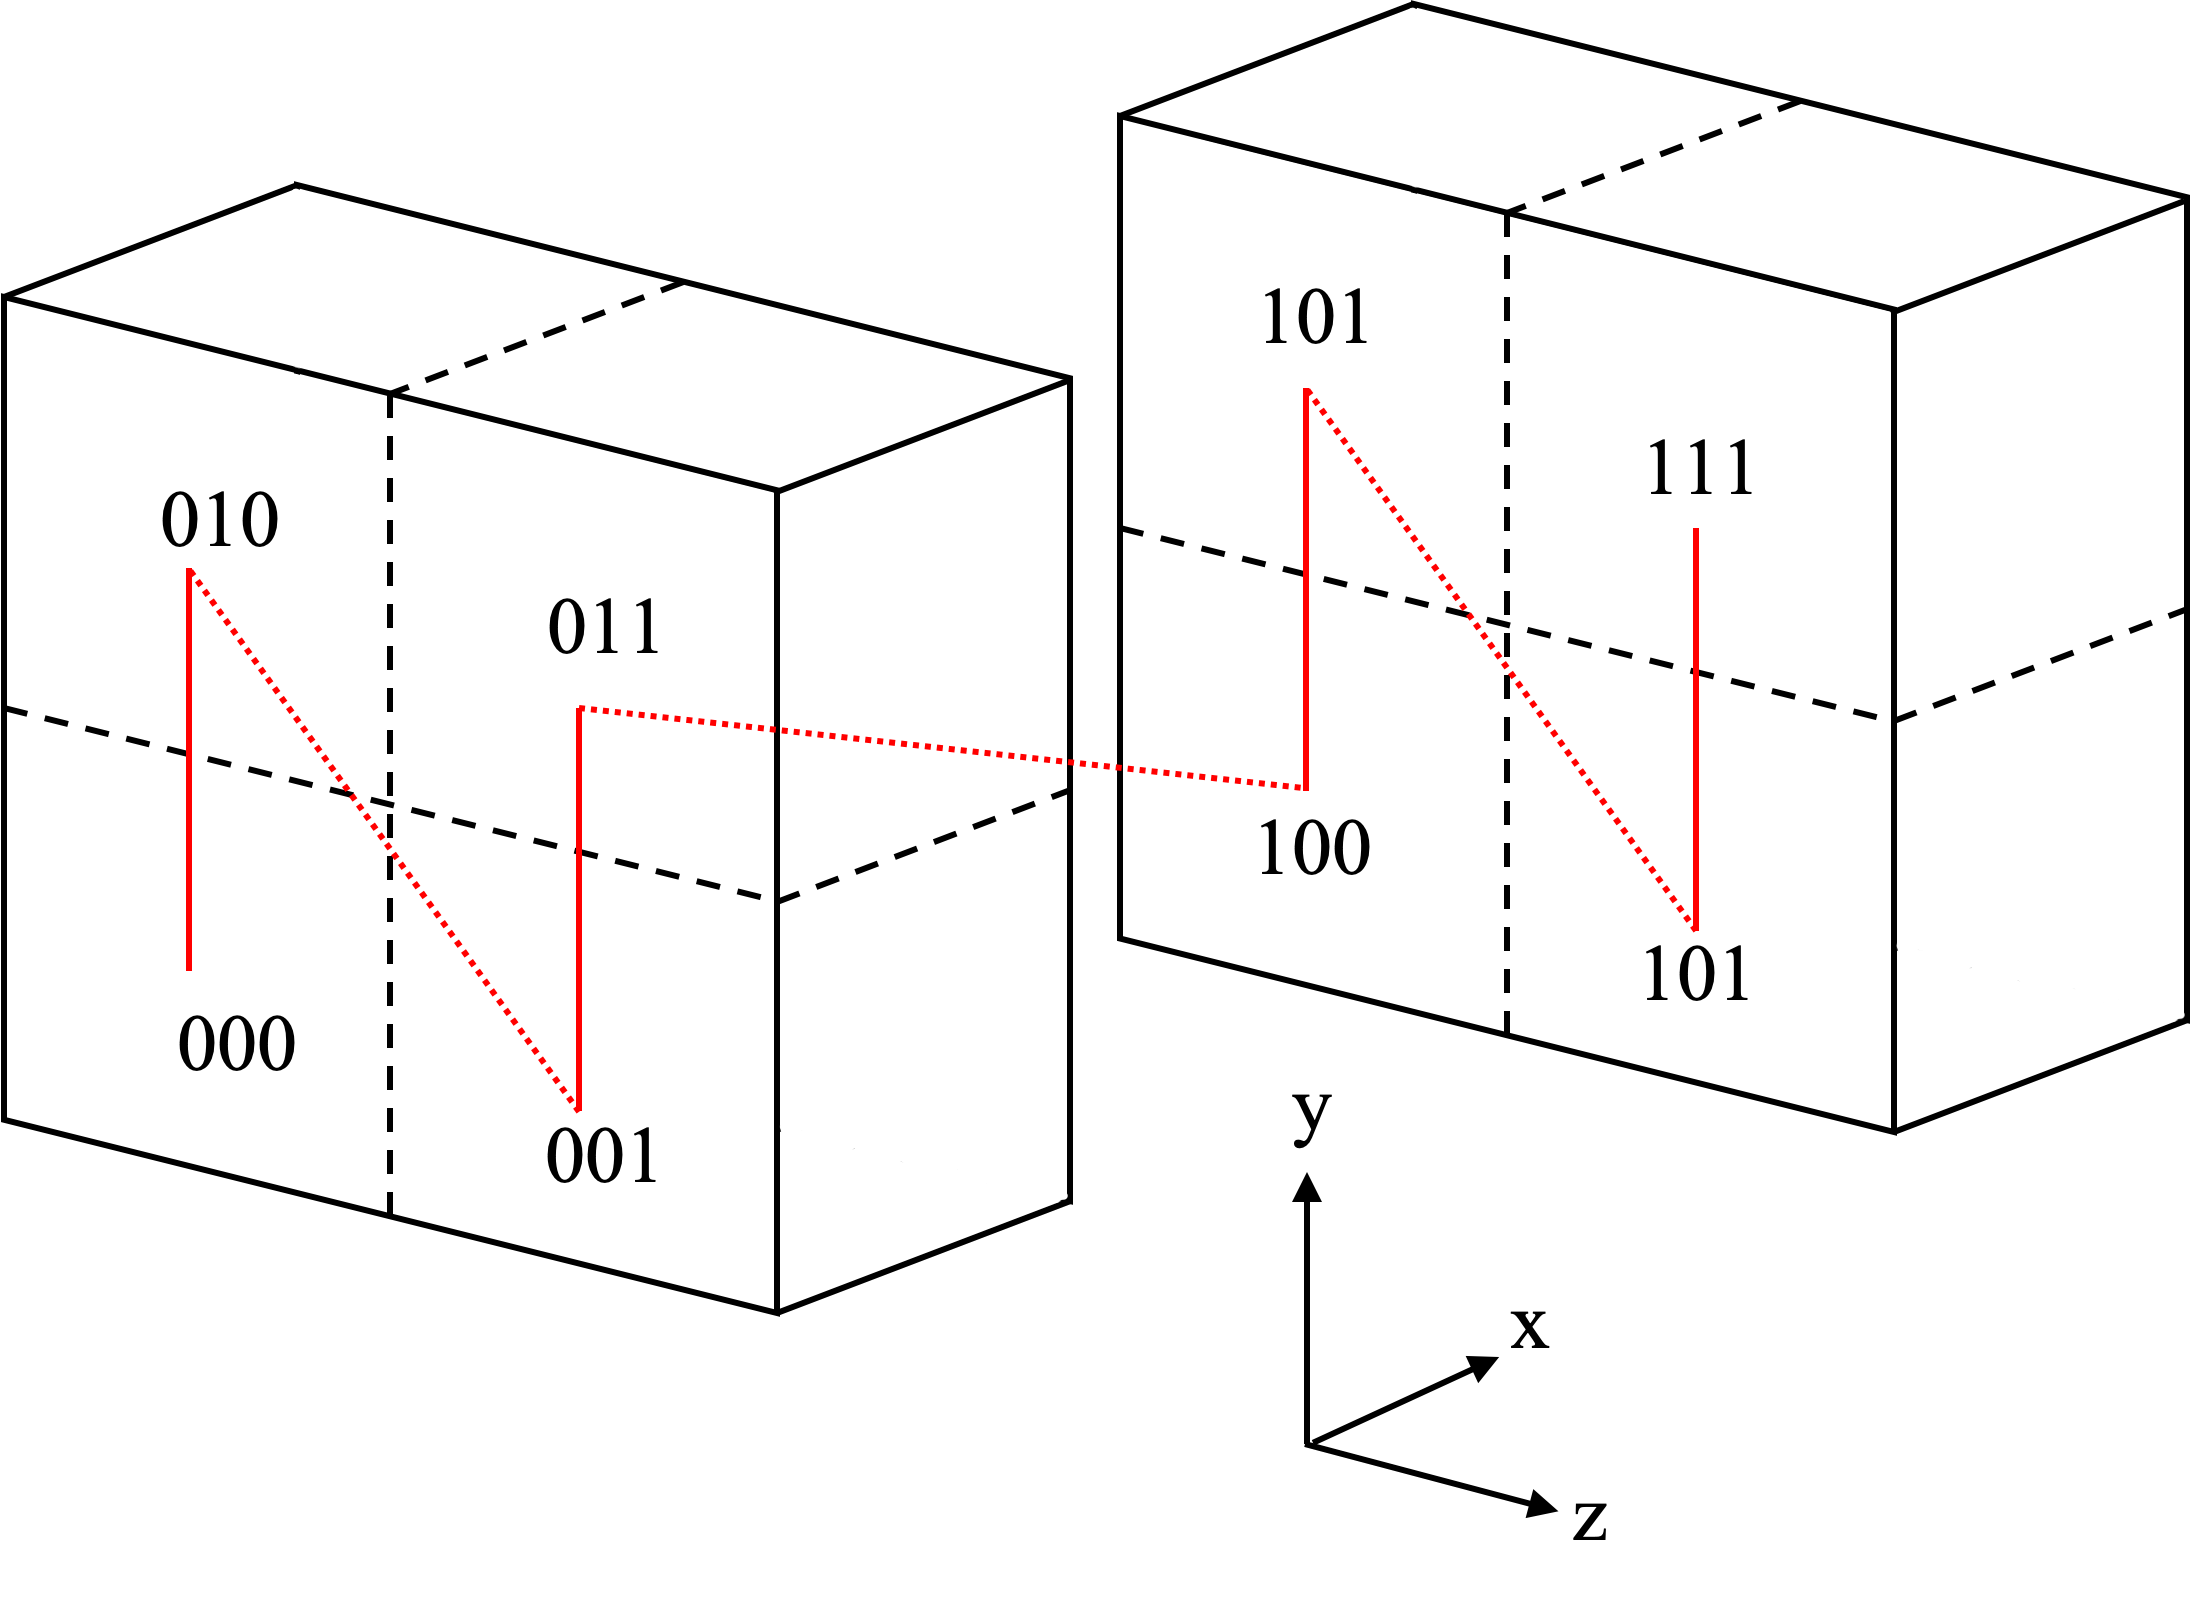
\includegraphics[width=0.65\textwidth]{chapter2/z_encoding.png}}
    \vspace{0pt}
    \caption{
        Morton encoding at level 1 of domain described by an non-adaptive octree.
        The two `layers' of the octree at this level have been broken apart
        in order to illustrate the encoded line. The Morton keys are written
        as binary coordinates in each octant.
    }
    \label{fig:2_2_morton_encoding}
\end{figure}